\hsection{Functions}%
%
Functions are blocks of code that can be invoked from anywhere else in a program.
You already learned many functions, from the basic \pythonilIdx{print} routine that just prints the value of its parameter to the output to the \pythonilIdx{sqrt} function from the \pythonilIdx{math} module which computes the square root.
Now you will learn how to make your own functions.%
%
\hsection{Defining and Calling Functions}%
\label{sec:definingFunctions}%
%
\pythonIdx{def}\pythonIdx{function!def}%
The syntax for defining our own functions in \python\ is as follows:%
%
\begin{pythonSyntax}
def my_function(param_1: type, param_2: type, ...) -> result_type:
    """
    Short sentence describing the function.

    The title of the so-called docstring is a short sentence stating
    what the function does. It can be followed by several paragraphs of
    text describing it in more detail. Then follows the list of
    parameters, return values, and raised exceptions (if any).

    :param param_1: the description of the first parameter (if any)
    :param param_2: the description of the second parameter (if any)
    :returns: the description of the return value (unless `-> None`).
    """
    body of function 1
    body of function 2
    return result  # if result_type is not None we return something


normal statement 1
normal statement 2
my_function(argument_1, argument_2)  # we can call the function like this
\end{pythonSyntax}
%
\pythonIdx{function!def}A function in \python\ is created by using the \pythonilIdx{def}\pythonIdx{function!def} keyword, followed by the name of the function.%
%
\bestPractice{functionNames}{Function names should be lower case, with underscores separating multiple words if need be~\cite{PEP8}.}%
%
\pythonIdx{function!parameter}Then follows an opening and a closing parenthesis, i.e., \pythonil{(...)}\pythonIdx{(\idxdots)}.
A function can have parameters through which we can pass values to it.
Inside the function, these parameters act like variables.
The values of these variables can be passed in when we call (invoke, execute) the function.%
%
\begin{definition}[Parameter]\pythonIdx{function!parameter}%
A function \emph{parameter} is a variable defined inside the function that receives its value when the function is called.%
\end{definition}%
%
Notice that, just like variables, all such parameters should be annotated with \pglspl{typeHint}~(see \cref{sec:variableTypesAndTypeHints})~\cite{PEP3107}.
Functions can return results~(like the \pythonilIdx{sqrt} function of the \pythonilIdx{math} module does) or return nothing~(like \pythonilIdx{print}).
\pythonIdx{function!return value}If they return a result, the type of this result is specified via the \pgls{typeHint} \pythonil{ -> result_type}\pythonIdx{->}.
We refer to the parameters and the return type of a function as its \pgls{signature}\pythonIdx{function!signature}.
The function header ends with a colon~(\pythonilIdx{:}).%
%
\bestPractice{functionTypeHints}{\pythonIdx{function!type hint}%
All parameters and the return value of a function should be annotated with \pglspl{typeHint}~\cite{PEP3107}. %
From my perspective: \emph{A function without \pglspl{typeHint} is wrong.}%
}%
%
Then, indented by four spaces, follows the function body.%
%
\bestPractice{functionBodyIndentation}{The body of a function is indented with four spaces.}%
%
\pythonIdx{function!body}This can be an arbitrary block of code, which may contain all the things we already learned.
\pythonIdx{function!return}The function can, at any point, be left using the \pythonilIdx{return} statement.
If the function is supposed to return a value \pythonil{result}, then this is done via \pythonil{return result}.
Notice that, like the \pythonilIdx{break} statement in loops, we can place \pythonilIdx{return} at any location we want.
We can also have multiple \pythonilIdx{return} values at different places in the function.%
%
\begin{sloppypar}%
\pythonIdx{function!call}The function \pythonil{my_function} then can be called from anywhere in the code by writing \pythonil{my_function(value_1, value_2, ...)}, where \pythonil{value_1} is passed in as value of \pythonil{param_1}, \pythonil{value_2} is passed in as value of \pythonil{param_2}, and so on.
This follows the same pattern of function calls that we already used in many of our examples.%
\end{sloppypar}%
%
\begin{definition}[Argument]\pythonIdx{function!argument}%
An \emph{argument} is the actual value given for a function parameter when the function is called.%
\end{definition}%
%
\pythonIdx{function!docstring}\pythonIdx{str!doc!function}%
Between the header of a function and its body, we always need to place a so-called \pgls{docstring}, which is a multi-line string~(see \cref{sec:multiLineStrings}).
This string consists of a title line shortly describing what the function does.
After an empty line, we can (but not necessarily need to) place a paragraph of text providing a more detailled discussion.
Then follows the list of parameters, each in the syntax \pythonil{:param parameter_name: description}\pythonIdx{:param:}.
Then follows the return value description (if the function returns something) in the form \pythonil{:returns: description}\pythonIdx{:returns:}.%
%
\bestPractice{funcDocstrings}{%
Each function should be documented with a \pgls{docstring}. %
If you work in a team or intend to place your code in public repositories like on \pgls{github}, then this very very much increases the chance that your code will be used correctly. %
From my perspective: \emph{A function without \pgls{docstring} is wrong.}%
}%
%
\bestPractice{functionSpace}{%
After the function and its body are defined, leave \emph{two} blank lines before writing the next code~\cite{PEP8}.%
}%
%
\gitPythonAndOutput{\programmingWithPythonCodeRepo}{05_functions}{def_factorial.py}{--args format}{functions:def_factorial}{%
Implementing a function computing the factorial of a positive integer number.}%
%
After all of this long introduction, let us finally come to some example.
Let's implement the factorial function as, well, function.
The factorial is defined as follows~\cite{D1991TEHOTFF,CB2022FBDOTFF}%
%
\begin{equation}%
\factorial{a}=\left\{\begin{array}{rl}%
1&\textnormal{~if~}a = 0\\%
\prod_{i=1}^a i&\textnormal{~otherwise, i.e., if~}a>0%
\end{array}\right.%
\label{eq:factorial}%
\end{equation}%
%
where $\prod_{i=1}^a i$ stands for the product~$1*2*3*\dots*(a-1)*a$.
We will implement this function in \python\ call it \pythonil{factorial} in \cref{lst:functions:def_factorial}.
It should take a single parameter~\pythonil{a} as parameter.
\pythonil{a} will be type-hinted as integer and the result of our function will be an integer as well.

The body of this function is straightforward.
We begin by initializing a variable \pythonil{product} with the value~\pythonil{1}.
Then, we need a loop that iterates a variable~$i$ over all integers less than or equal to~\pythonil{a}.
We want to multiply these values to~\pythonil{product}.
Well, we can skip over~$\pythonil{i}=1$, because that would be useless.
So we will use a \pythonilIdx{for} loop iterating~\pythonil{i} over the \pythonil{range(2, a + 1)}\pythonIdx{range}.
This effectively starts~\pythonil{i} at~\pythonil{2}.
Since the upper limit~\pythonil{a + 1} of the \pythonilIdx{range} is always \emph{exclusive}, the last value for~\pythonil{i} will be~\pythonil{a}.
Notice that we really use \pythonil{a} like a normal variable that was assigned a value.%
%
\begin{sloppypar}%
Anyway, inside the loop body, we compute \pythonil{product *= i}\pythonIdx{*=}, which is equivalent to \pythonil{product = product * i}.
After the loop, \pythonil{product} holds $\factorial{\pythonil{a}}$.
So we can return it as the result of the function, by writing \pythonil{return product}\pythonIdx{return}.%
\end{sloppypar}%
%
We can now compute the factorial of any number~\pythonil{x} by calling~\pythonil{factorial(x)}.
After the function body, we leave two empty lines.
And then we compute the factorials of the numbers from~$1$ to~$9$ in a \pythonilIdx{for}-loop and print them by using \pglspl{fstring}.
Inside this loop and in the \pgls{fstring}, we can use the function \pythonil{factorial} exactly like any other function we used before, like \pythonil{sqrt} or \pythonil{print}.
It may be an interesting side information at the end of this example that the factorial can actually be computed \emph{faster} than using this product form, see, e.g.~\cite{L2015ANKOFF}.

\gitPythonAndOutput{\programmingWithPythonCodeRepo}{05_functions}{def_gcd.py}{--args format}{functions:def_gcd}{%
Implementing the Euclidean Algorithm as a function and calling it from another function.}%

Functions can have a more than one parameter or no parameter at all.
They can return one value or return nothing at all.
Functions can also be called from other functions.
Let us investigate these options by investigating another interesting mathematical operation:
The computation of the greatest common divisor, also known as~\pythonil{gcd}.

This can be done using the Euclidean algorithm~\cite{EHF2008ENT,B1999FAOTBEA,TKY2016BEOEAOTCEG}, going back to \citeauthor{EHF2008ENT} who flourished about 300~BCE.
The greatest common divisor of two numbers positive~$a\in\naturalNumbersO$ and~$b\in\naturalNumbersO$ is the greatest number~$g\in\naturalNumbersO=\pythonil{gcd}(a,b)$ such that~$a\bmod g=0$ and~$b \bmod g=0$, where~$\bmod$ is the \pgls{modulodiv} operator equivalent to \python's~\pythonilIdx{\%}.
This means that $g$~divides both $a$ and $b$ without remainder.
If $a=b$, then obviously $\pythonil{gcd}(a,b)=a=b$ as well.
Otherwise, we know that $a=ig$ for some~$i\in\naturalNumbersO$ and $b=jg$ for some~$j\in\naturalNumbersO$.
If we assume, without loss of generality, that~$a>b$.
Then, $c=a-b=(i-j)g$ and it will be clear that $c\bmod g=(a-b)\bmod g=(i-j)g\bmod g = 0$ as well, i.e., that $\pythonil{gcd}(a,b)=\pythonil{gcd}(a-b, b)=g$.
Similarly, $d=a\bmod b=ig\bmod (jg)=ig-\lfloor i/j\rfloor*jg=g(i-j\lfloor i/j\rfloor)$ is still divisible by~$g$ without remainder as~$d\bmod g=0$.
This means that~$\pythonil{gcd}(a\bmod b, b)=\pythonil{gcd}(a, b)=g$, too.

Since both~$d$ and~$c$ are less than~$a$, we could replace~$a$ with either of them.
In particular, $d$~will be less than both~$a$ and~$b$, so we could store~$b$ in~$a$ and replace~$b$ with~$d$.
We would repeat the computation until reaching~$b=0$, at which point~$a$ will be~$g$.
Matter of fact, by choosing the module-based update, we do not even need to assume that~$a>b$.
Because if~$b>a$, then~$a \bmod b=a$ and we would just switch~$a$ and~$b$ in this step.
If~$a=b$, then~$a \bmod b=0$ and we would immediately terminate after the first step and return~$a$ as the greatest common divisor.

This algorithm is implemented in \cref{lst:functions:def_gcd} as function~\pythonil{gcd}.
\pythonil{gcd} has two integer parameters, \pythonil{a} and~\pythonil{b}, and returns another~\pythonil{int}.
Its body is surprising short:
We use a \pythonilIdx{while} loop that iterates as long as \pythonil{b > 0}.
After the loop, we \pythonil{return a}\pythonIdx{return} as the result.
If \pythonil{b == 0} holds at the beginning, the loop will never be executed and~\pythonil{a} is returned as-is, which is correct:
$\pythonil{gcd}(a, 0)=a$ for all~$a\in\naturalNumbersO$.

However, if \pythonil{b > 0}, we enter the loop's body, which is a single line of code:
the tuple-unpacking command~\pythonil{a, b = b, a \% b}~(see \cref{sec:lists}).\pythonIdx{tuple!unpacking}\pythonIdx{unpacking}
This line first completely evaluates the right-hand side.
This creates a tuple\pythonIdx{tuple} where the first value is~\pythonil{b}.
The second value is~\pythonil{a \% b}.
The tuple is then unpacked and stored in the variables~\pythonil{a} and~\pythonil{b}.
\pythonil{a} will thus receive the value that \pythonil{b}~had during the evaluation of the right-hand side.
\pythonil{b} will receive the previously computed value of~\pythonil{a \% b}.
In other words, \pythonil{b} is stored in~\pythonil{a} and the remainder of the division of \pythonil{a} by \pythonil{b} is stored in~\pythonil{b}.
Clearly, \pythonil{b} will become smaller in each iteration and since it can never become negative, it will eventually reach~\pythonil{0} and the loop will terminate.
Similarly, the \pythonil{gcd} is never \inQuotes{lost} during the loop and will thus be the value in~\pythonil{a} at the end.
And this value is returned.

So this was a function with two parameters and one return value.
Let us now implement a second function, this time with no return value.
\pythonil{print_gcd} accepts again two parameters~\pythonil{a} and~\pythonil{b} and returns nothing.
Instead, it will print the \pythonil{gcd} nicely using \pythonilIdx{print} and an \pgls{fstring}.
Since the \pythonilIdx{math} module also provides a function names \pythonilIdx{gcd} for computing, well, the greatest common divisor, we want to compare the result of our function with this one.%
%
\begin{sloppypar}\pythonIdx{function!import}%
Of course, we cannot have two functions named \pythonil{gcd} in the same context.
So we import the function from the \pythonilIdx{math} module \emph{under a different name}:
\pythonil{from math import gcd as math_gcd}\pythonIdx{as}\pythonIdx{import}\pythonIdx{from} makes the \pythonilIdx{gcd} function from the module \pythonilIdx{math} available under the name~\pythonil{math_gcd}.
And we use it in the \pgls{fstring} in \pythonil{print_gcd} under that name.%
\end{sloppypar}%
%
Finally, we confirm that \pythonil{gcd} and \pythonil{math_gcd} compute the same result for four test cases at the bottom of our program.
Now that all is said and done, it should be mentioned that the Euclidean Algorithm has a particularly efficient binary variant which is faster than our implementation in \cref{lst:functions:def_gcd}.
This binary variant may have been developed in China in the first century~CE~\cite{B1999FAOTBEA}.%
%
\FloatBarrier%
\endhsection%
%
\hsection{Functions in Modules}%
\label{sec:functionsInModules}%
\pythonIdx{module!import}\pythonIdx{function!import}\pythonIdx{function!module}%
%
\gitPython{\programmingWithPythonCodeRepo}{05_functions/my_math.py}{--args format}{functions:my_math}{%
The module \pythonil{my_math}, which provides two mathematics functions, namely \pythonil{sqrt}, implementing the algorithm of Heron to compute the square root from \cref{lst:loops:while_loop_sqrt}, and \pythonil{factorial}, copied from \cref{lst:functions:def_factorial}.}%
%
You may not have noticed it, but we just made a very big step in our programming skills.
We moved from simple programs which only consist of one big block of code to modular programs.
We can now reuse code.
And we can distribute code over multiple files.
This clearly is a concern for any application larger than a simple script:
How can we avoid writing our applications as a single, huge, and unstructured file which would be impossible to maintain in the long run?
How can we divide our application into smaller units that we can test, improve, and maintain separately and maybe use and reuse in different contexts?
A big part of the answer to this question are \emph{modules} and \emph{packages}~\cite{PSF2024TIS}.

For all intents and purposes within this book, a \emph{module}\pythonIdx{module} is a \python\ file and a \emph{package}\pythonIdx{package} is a directory wherein the file is located.
As described in~\cite{PSF2024TIS}, modules do not necessarily need to be files and packages can probably be created otherwise as well, but let us keep it simple here.

Indeed, we have already worked with modules, most prominently the~\pythonilIdx{math} module.
This module is basically a collection of mathematical functions.
Since we have implemented several mathematical functions by ourselves, let us put some of them in a module as well.

In \cref{lst:functions:my_math} we do just that.
We create the \python\ file \textil{my_math.py} and place two functions into it:
The function \pythonil{factorial} from \cref{lst:functions:def_factorial} and a new function called \pythonil{sqrt}.
The \pythonil{sqrt} function basically encapsulates our code from back in \cref{lst:loops:while_loop_sqrt}, where we implemented the Heron's Method to compute the square root, as a function.
Now, \pythonil{number}, the input of this algorithm, comes in as a parameter.%
%
\bestPractice{packageAndModuleNames}{Package and module names should be short and lowercase. Underscores can be used to improve readability.~\cite{PEP8}}%
%
Our new module \textil{my_math} does not look very special or different from what we did so far.
The one difference that we notice, however, is that it \inQuotes{does nothing}.
In the file, we define two functions, but we do not actively call them, we do not use them for anything.
This is the purpose of this module:
It just provides the functions.
We will use them elsewhere.

\gitPythonAndOutput{\programmingWithPythonCodeRepo}{05_functions}{use_my_math.py}{--args format}{functions:use_my_math}{%
A program using the functions \pythonil{sqrt} and \pythonil{factorial} from the module \pythonil{my_math} given in \cref{lst:functions:my_math}.}%%
%
\begin{sloppypar}%
\Cref{lst:functions:use_my_math} is where we use them:
We write a program, i.e., another \python\ file, named \textil{use_my_math.py}.
In this file, we want to use our two functions \pythonil{factorial} and \pythonil{sqrt} from the module \pythonil{my_math}.
For this purpose, we have to tell the \python\ interpreter where it can find these two functions.
We do this by writing \pythonil{from my_math import factorial, sqrt}\pythonIdx{from}\pythonIdx{import}\pythonIdx{module}.
The meaning of the line is quite obvious:
There is a module \pythonil{my_math} from which we want to import, i.e., make available, two functions, namely \pythonil{factorial} and \pythonil{sqrt}.%
\end{sloppypar}%
%
Now, the \python\ interpreter knows a lot of modules.
Several modules ship with any \python\ installation, like \pythonilIdx{math}.
Others are installed via a package manager like \pgls{pip}~\cite{PSF2024IPM} (we will eventually discuss this later).
The \pythonil{my_math} module is found because it is in the same directory as the program \textil{use_my_math}.

If we had placed the \textil{my_math.py} file into a sub-directory named \textil{math_pack} instead, then we would import our functions from \textil{math_pack.my_math} instead, where \textil{math_pack} would be called a~\emph{package}.
Of course, we could also create another level of directories, say we could have directory \textil{utils}, containing directory \textil{math_pack}, containing our file \pythonil{my_math.py}.
In this case, we would import our functions like \pythonil{from utils.math_pack.my_math import}\dots.
The names of package and modul are separated by a~\pythonilIdx{.} when importing from them.
This allows us to nicely and hierarchically structure our projects into modules and packages for different purposes.

In \cref{lst:functions:use_my_math} we can use both \pythonil{sqrt} and \pythonil{factorial} exactly as if we had defined them in this program.
We first print a few values for \pythonil{sqrt} and \pythonil{factorial} and also show that we can compute the result of the square root of a factorial.
We also just copy the code from \cref{lst:loops:for_loop_pi_liu_hui}, where we use LIU Hui's method to approximate~\numberPi\ -- but this time, we use our own implementation of the square root function instead of the one from the \pythonil{math} module.
Interestingly, the sixth and last approximation step in \cref{exec:functions:use_my_math} shows exactly the same result as in \cref{exec:loops:for_loop_pi_liu_hui}.%
%
\FloatBarrier%
\endhsection%
%
\hsection{Interlude:~Unit Testing}%
\label{sec:unitTesting}%
\pythonIdx{function!unit test}%
\pythonIdx{function!testing}%
%
Structuring our code into functions and modules has several advantages.
We can reuse code and we can divide big application into smaller pieces, both of which make it easier to understand what our program is doing.
Or is \emph{supposed} to be doing.
Because errors happen in programming.
They happen often and they happen naturally.

But dividing code into functions and placing it into modules has yet another advantage:
We can test these separate functions separately.
Imagine that you have a big application using lots of components, code for reading and writing files, code for making mathematical computations, and so on.
It is not eay to figure out how to check that the big application behaves exactly as it is supposed to.
There will be many combinations of inputs and environments and conditions that we would need to test.
Even if we would find that the application behaves, maybe only in some cases, a bit strange, it would be hard to figure out which of its many components has an error.

However, we can also do something else:
We can test each component separately, too.
It is much easier to check whether our \pythonil{factorial} and \pythonil{sqrt} functions behave as we expect them than to do this for a whole complex program.%
%
\begin{definition}[Unit Testing]
\emph{Unit Testing} is a software testing technique where separate components or functions of an application are tested in isolation.
\end{definition}%
%
The goal of unit testing is to ensure that each unit of the software performs as expected.
Since tests can be developed along (or even before!) the single functions are implemented, potential errors can be found early in the development process.
As the unit tests focus on smaller, well, units, they can be less complex and easier to understand.
The consequent usage of unit tests supports a modular and cleaner programming style, as it forces the developer to divide bigger programs into smaller pieces that can be invoked and tested in separation.
Finally, unit testing is especially useful if an application is developed, improved, and maintained over a long time:
If test cases are preserved and re-tested every time the software changes, then we can discover if a change that we applied to an older piece of code breaks a unit test, i.e., may lead to an unwanted change of behavior our program that we did not anticipate.
Especially with its increased automation, unit testing in software development has steadily gained importance during the past decades~\cite{W2000WISTAWIISH,TLG2006UTCU,R2006ASOUTP} and is an important cornerstone of \python\ software development~\cite{P2021PUTAAOAEUTIP,O2022PTWP,DG2020TIP}.%
%
%
\begin{figure}%
\centering%
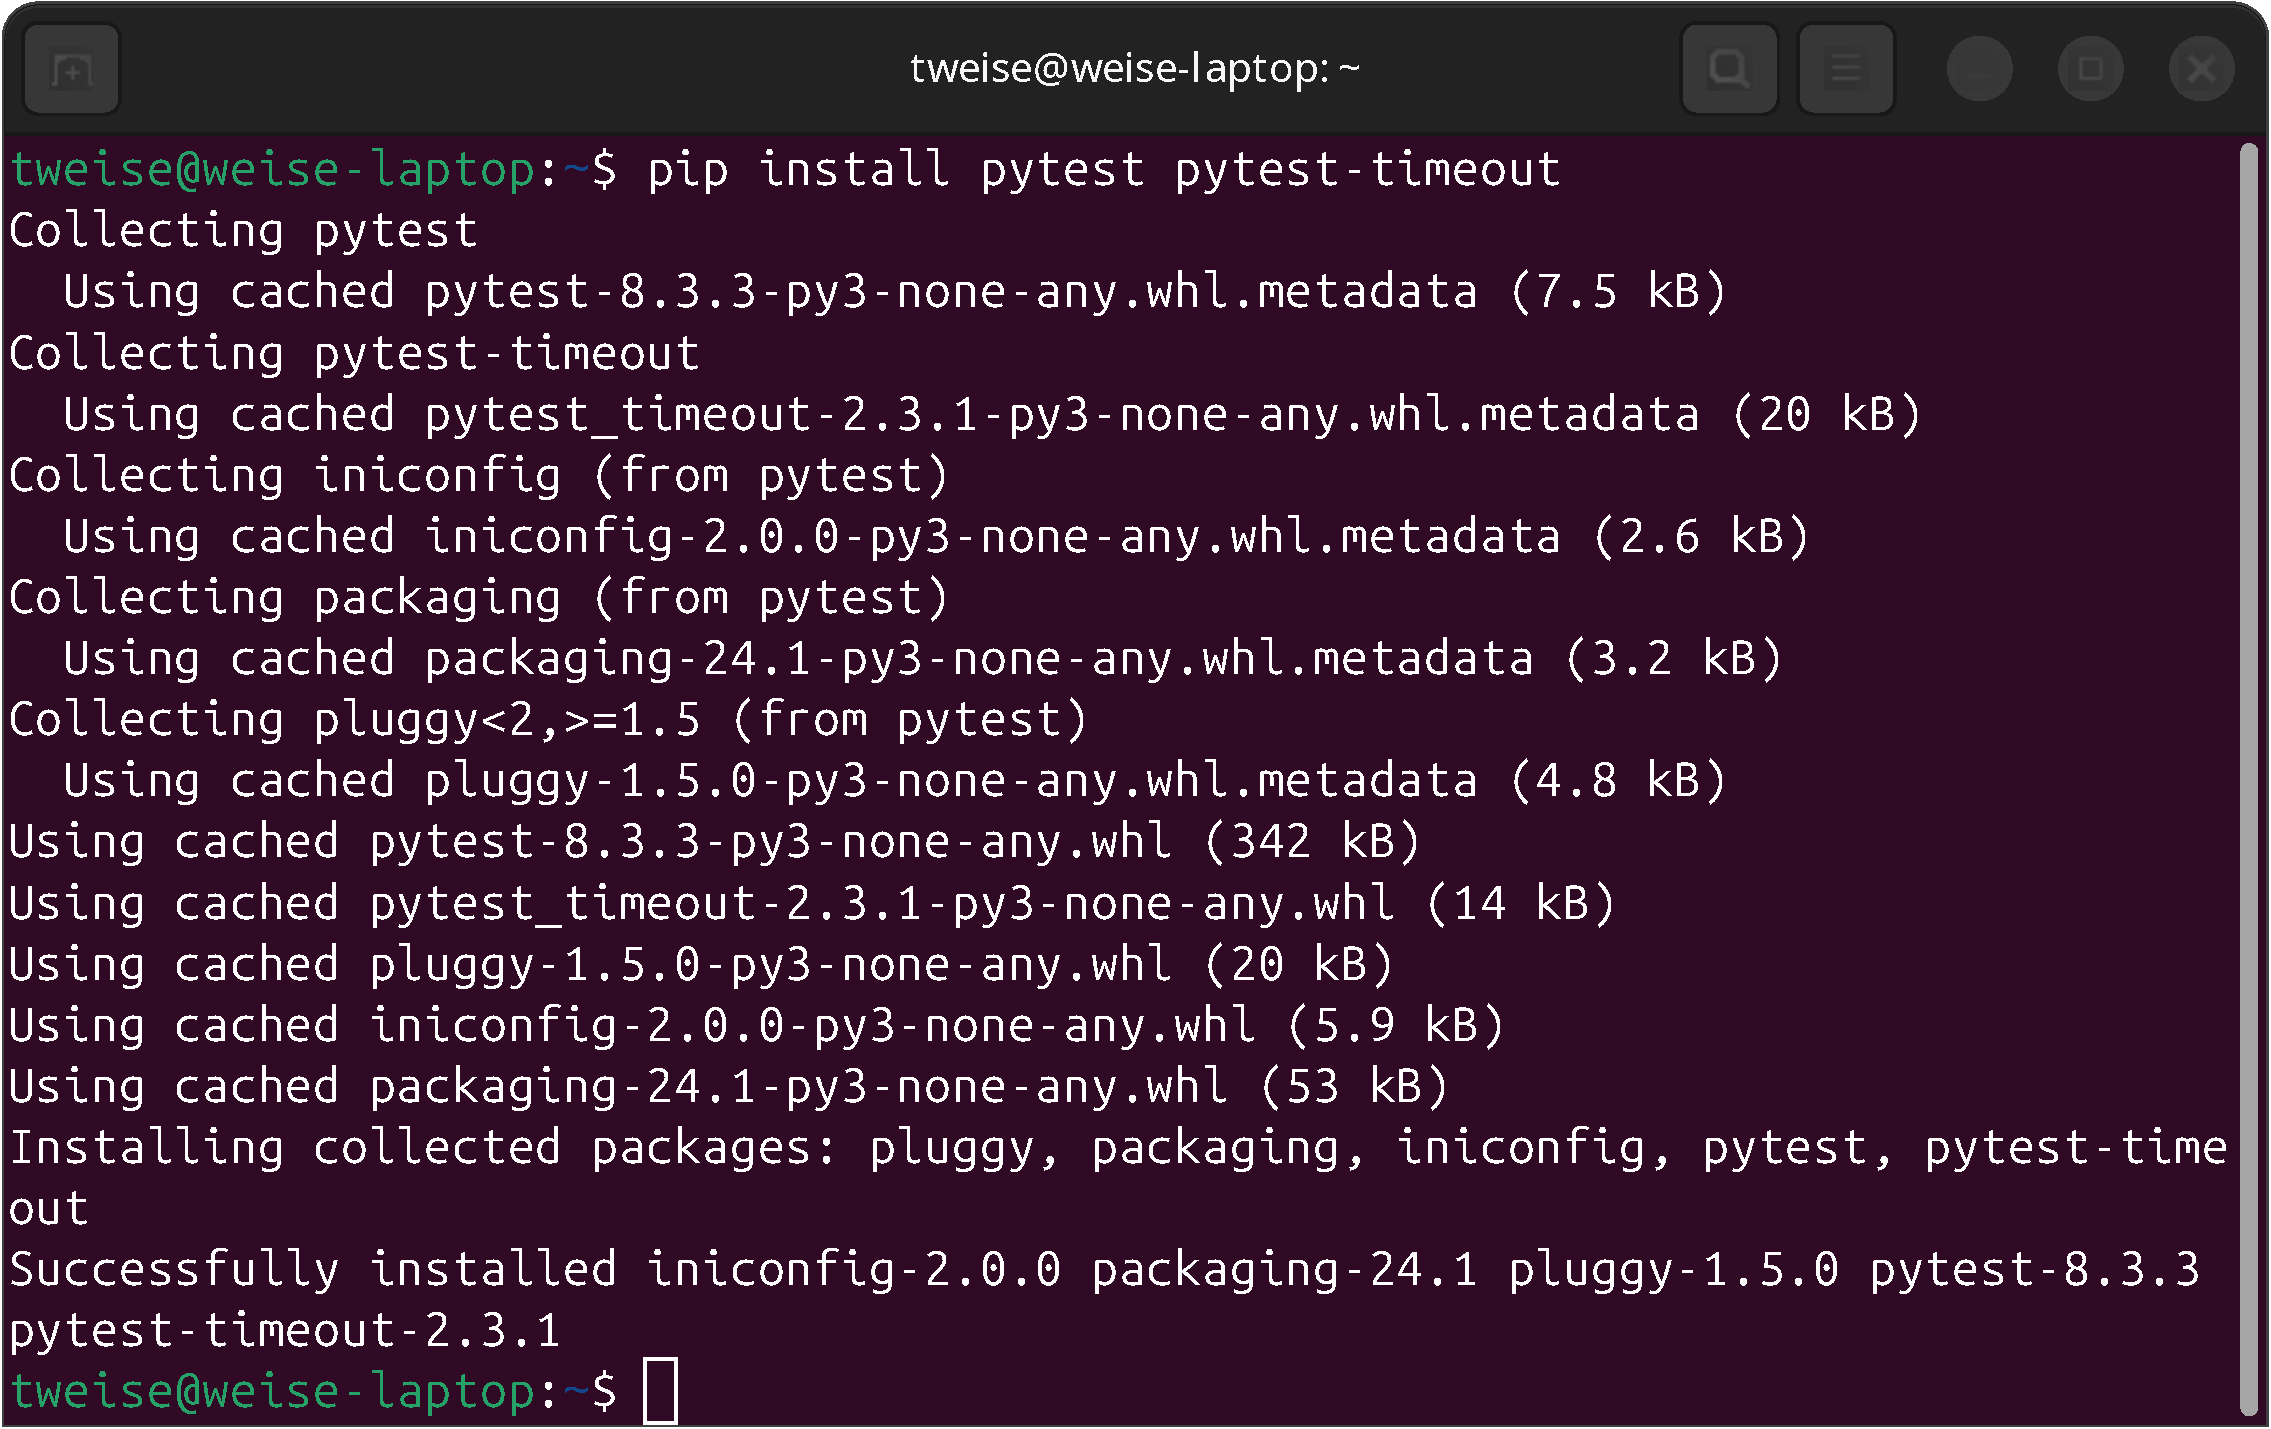
\includegraphics[width=0.7\linewidth]{\currentDir/pipInstallPytest}%
\caption{Installing \pytest\ in a \ubuntu\ \pgls{terminal} via \pip~(see \cref{sec:pipAndVenv} for a discussion of how packages can be installed).}%
\label{fig:pipInstallPytest}%
\end{figure}%
%
\usefulTool{pytest}{%
\pytest\ is a \python\ is a \python\ framework for writing and executing software tests~\cite{KPDT2024PD}.
It can be installed via \bashil{pip install pytest pytest-timeout} as shown in \cref{fig:pipInstallPytest} on \cpageref{fig:pipInstallPytest}. %
You can then apply \pytest\ using the command \bashil{pytest --timeout=toInS file(s)}, where \textil{toInS} should be replaced with a reasonable timeout in seconds and \textil{file(s)} is one or multiple files with test cases. %
We provide a script for using \pytest\ with a reasonable default configuration in \cref{lst:bash:pytest} on \cpageref{lst:bash:pytest}. %
See also \cref{ut:doctest} later on.%
}%
%
You will ask yourself how testing and especially the reuse of test cases works.
It is, actually, fairly simple:
We have our actual program code in one or multiple \python\ files.
We have our test code in some other \python\ files.
For the same of clarity, if the actual code is in a file~\textil{my_code.py}, then we could the code for the tests into a file called~\textil{test_my_code.py}.

\gitPython{\programmingWithPythonCodeRepo}{05_functions/test_my_math.py}{--args format}{functions:test_my_math}{%
A small unit test suite for \cref{lst:functions:my_math}.}%
%
\gitOutputTool{\programmingWithPythonCodeRepo}{.}{scripts/pytest.sh 05_functions test_my_math.py}{functions:test_my_math:pytest}{%
The output of the unit tests in \cref{lst:functions:test_my_math}: While the test of \pythonil{factorial} succeeds, our \pythonil{sqrt} function fails for input~\pythonil{0.0}.}%

In \cref{lst:functions:test_my_math} we do just that.
We create a file \textil{test_my_math.py} and into this file, we want to put the code for testing our module~\textil{my_math}.
This testing code is defined in form of functions.
The names of these functions must start with \textil{test_}.

Now our module \textil{my_math} provides two functions, \pythonil{factorial} and \pythonil{sqrt}.
At the top of our new tests module \textil{test_my_math}, we \pythonilIdx{import} both of these functions.
Naturally, we would create corresponding test functions and call them \pythonil{test_factorial} and \pythonil{test_sqrt}.
These functions have no parameters and no return values.

Tests are often defined in the form of several assertions assertions:\pythonIdx{assert}%
%
\begin{pythonSyntax}
assert booleanExpr  # raises AssertionError if not booleanExpr
\end{pythonSyntax}
%
An assertion is defined by the keyword \pythonilIdx{assert} followed by an arbitrary Boolean expression.
If the Boolean expression evaluates to \pythonil{True}, then nothing happens.
If it evaluates to \pythonil{False}, then an \pythonilIdx{AssertionError} is raised.
This error will cause the test function to fail immediately.
We will learn in \cref{sec:exceptions} what \pythonilsIdx{Exception} are and how to handle them in detail.
If the complete test function runs through without raising any \pythonilIdx{Exception}, then the test has succeeded.
If it fails or raises an \pythonilIdx{Exception} at any point during its execution, the test has failed.

Now we create the function \pythonil{test_factorial} to test the \pythonil{factorial} function.
For example, we know that $\factorial{0}=1$.
So it makes sense to define \pythonil{assert factorial(0) == 1}.
The Boolean expression here is \pythonil{factorial(0) == 1}, which is obviously only \pythonil{True} if \pythonil{factorial(0)} evaluates to~\pythonil{1}.
We define similar cases for~\factorial{1}, \factorial{2}, and~\factorial{3}.
Obviously, we cannot write down a complete list of all possible inputs.
But these are the four smallest ones for which the factorial is defined.
By testing also \factorial{12}, we have checked \pythonil{factorial} for a mid-sized argument.
We then also create a test case for a fairly large number, say~\factorial{30}.
We have computed this value using an online tool that offers arbitrary precision.
The result of this function is more than~$265*10^{30}$, which is fairly beyond the range of 64~bit integers (and thus showcases that integers in \python~3 have an unlimited range, as stated back in \cref{sec:int}).
This test case validates whether our \pythonil{factorial} function works well for large numbers, too.
If our \pythonil{factorial} function passes all of these tests, we can be fairly certain that it is implemented correctly.
There could still be errors, though.
For example, we did not test~\factorial{4}.
But at least it looks unlikely that~\factorial{3} and~\factorial{12} \inQuotes{work,} but not~\factorial{4}.

For the \pythonil{sqrt} function, we create similar test function and call it \pythonil{test_sqrt}.
Reasonable test cases are \pythonil{assert sqrt(0.0) == 0.0}, \pythonil{assert sqrt(1.0) == 1.0}, and \pythonil{assert sqrt(4.0) == 2.0}.
We would also expect that \pythonil{sqrt(x) * sqrt(x) == x} for different~\pythonil{x}.
However, we have to account for the limited precision of the datatype \pythonilIdx{float} discussed in \cref{sec:howFloatingPointNumbersWork}.
Even if we would get as close to \pythonil{sqrt(x)} for some~\pythonil{x} as possible, we can only represent 15 to 16 digits.
Therefore, we have to give a little bit of wiggle room when we compute \pythonil{s3 = sqrt(3.0)} and expect that \pythonil{s3 * s3 == 3.0}.
We do this by writing \pythonil{assert abs(s3 * s3 - 3.0) <= 5e-16}, i.e., by assuming that the difference between \pythonil{3.0} and \pythonil{s3 * s3} is not bigger than the very small number~$5*10^{-16}$.
On the other hand, the square root of \pythonil{1e10 * 1e10} should be representable exactly, namely as~\pythonil{1e10}.

The datatype \pythonilIdx{float} also offers us two special values, which both can be imported from the \pythonilIdx{math} module and which were discussed in \cref{sec:float:special}:
\pythonilIdx{inf} stands for positive infinity~$+\infty$ and \pythonilIdx{nan} stands basically for \inQuotes{undefined}, a value that you may get if you try to compute something like~\pythonil{inf - inf}.
Our \pythonil{sqrt} function has to understand and correctly handle these values as well.
\pythonil{sqrt(inf)} should again return~\pythonilIdx{inf}.
\pythonil{sqrt(nan)} should return~\pythonil{nan}.
However, we cannot do \pythonil{assert sqrt(nan) == nan}, since \pythonilIdx{==} will yield \pythonil{False} for any value if at least one \pythonilIdx{nan} is involved (see again \cref{sec:float:special}).
For testing whether \pythonil{sqrt(nan)} yield~\pythonilIdx{nan}, we use the function~\pythonilIdx{isnan} from the \pythonilIdx{math} module.
This function returns \pythonil{True} for \pythonil{isnan(nan)} and \pythonil{False} otherwise.

With this, we have covered most reasonable inputs that either \pythonil{factorial} or \pythonil{sqrt} could receive.
We have defined what we would expect as output for these inputs.
These expectations are implemented as test cases.
Regardless of how \pythonil{factorial} or \pythonil{sqrt} are implemented, they should pass these test cases.
Otherwise, they are wrong.

Running our test cases with \pytest\ yields the output in \cref{exec:functions:test_my_math:pytest}.
This output tells us that \pythonil{test_factorial} ran through without any issue.
\pythonil{test_sqrt} however failed with a \pythonilIdx{ZeroDivisionError} that was raised inside our \pythonil{sqrt} function.
This happened when we tried to compute~\pythonil{sqrt(0.0)}.

When we look back at our \pythonil{my_math} module in \cref{lst:functions:use_my_math}, we find that our initial guess for the square root is~\pythonil{1}.
In each step, we then compute \pythonil{guess = 0.5 * (guess + number / guess)}.
If \pythonil{number} is \pythonil{0.0}, then this effectively means \pythonil{guess = 0.5 * guess}.
We have learned that the precision of \pythonilsIdx{float} is finite and that positive values smaller than \pythonilIdx{5e-324}\pythonIdx{float!smallest} will just become~\pythonil{0.0}.
This will happen here too, and \pythonil{guess} will thus eventually become~\pythonil{0.0}.
In the next iteration, this leads to us trying to divide~\pythonil{0.0 / 0.0}, causing the \pythonilIdx{ZeroDivisionError}.
%
\FloatBarrier%
\gitPython{\programmingWithPythonCodeRepo}{05_functions/my_math_2.py}{--args format}{functions:my_math_2}{%
An improved variant of \cref{lst:functions:my_math} dealing with the failing test case~\pythonil{0.0} discovered in \cref{exec:functions:test_my_math:pytest}.}%
%
\gitPython{\programmingWithPythonCodeRepo}{05_functions/test_my_math_2.py}{--args format}{functions:test_my_math_2}{%
We use the same small unit test suite given in \cref{lst:functions:test_my_math} for \pythonil{sqrt} in \cref{lst:functions:my_math_2}.}%
%
\gitOutputTool{\programmingWithPythonCodeRepo}{.}{scripts/pytest.sh 05_functions test_my_math_2.py}{functions:test_my_math_2:pytest}{%
The output of the unit tests in \cref{lst:functions:test_my_math_2}: This time, we hit the timeout because of an endless loop!}

In order to fix this problem, we introduce the check \pythonil{if number <= 0.0} into our \pythonil{sqrt} function in \cref{lst:functions:test_my_math_2}.
If this new conditional evaluates to \pythonil{True}, we return~\pythonil{0.0} directly.
Now we do not consider the case that a negative number is passed into \pythonil{sqrt} at this point.
Here, we would ideally \pythonilIdx{raise} an error by ourselves, but we will learn only later how to do that.\footnote{%
We learn it in \cref{sec:exceptions} and there we will revisit our \pythonil{sqrt} function in \cref{lst:exceptions:sqrt_raise}, too.}

We apply the same tests to the new version of the \pythonil{sqrt} function in \cref{lst:functions:test_my_math_2}.
The output of the test case, provided in \cref{exec:functions:test_my_math_2:pytest}, now indicates another error:
We a timeout!

You see, when invoking \pytest\ with the option \bashil{--timeout=10} -- which only works if the package \textil{pytest-timeout} is installed -- we limit the maximum runtime of our test suite to ten seconds.
Ten seconds is a reasonable time for \emph{this book} as we actually run all the scripts automatically during the book building process.
In practical situations, you will usually choose a larger time limit.%
%
\bestPractice{testTimeout}{%
Always attach a timeout to your unit tests. %
This timeout can be generous, maybe one hour, but it will serve as sentinel against either endless loops, deadlocks, or other congestion situations which all would be practical test failures. %
Timeouts protect automated builds or continuous integration systems from clogging.}%
%
\begin{sloppypar}%
The time limit protected us here.
Our \pythonil{sqrt} function goes into an endless loop if \pythonil{number = inf}.
Initially, we set \pythonil{guess = 1.0}.
In the first iteration of the loop in \pythonil{sqrt}, \pythonil{guess = 0.5 * (guess + number / guess)} makes \pythonil{guess} become \pythonil{inf}.
However, in the second iteration, we have \pythonil{number / guess} becoming \pythonil{inf / inf} which yields~\pythonil{nan}.
From now on, all calculations yields \pythonil{nan}.
Since \pythonil{nan != nan} is \pythonil{True}, the loop never ends.%
\end{sloppypar}%
%
\gitPython{\programmingWithPythonCodeRepo}{05_functions/my_math_3.py}{--args format}{functions:my_math_3}{%
An improved variant of \cref{lst:functions:my_math_2} dealing with the failing test case~\pythonilIdx{inf} discovered in \cref{exec:functions:test_my_math_2:pytest}.}%
%
\gitPython{\programmingWithPythonCodeRepo}{05_functions/test_my_math_3.py}{--args format}{functions:test_my_math_3}{%
We use the same small unit test suite given in \cref{lst:functions:test_my_math} for \pythonil{sqrt} in \cref{lst:functions:my_math_3}.}%
%
\gitOutputTool{\programmingWithPythonCodeRepo}{.}{scripts/pytest.sh 05_functions test_my_math_3.py}{functions:test_my_math_3:pytest}{%
The output of the successful unit tests in \cref{lst:functions:test_my_math_3}.}%
%
\begin{sloppypar}%
We finally solve this problem in \cref{lst:functions:my_math_3}.
Here, we add a new condition: \pythonil{if not isfinite(number)}, we return \pythonil{number} as-is.
\pythonilIdx{isfinite} is another function from the \pythonilIdx{math} module.
It takes one parameter and it returns \pythonil{True} if it is a finite number and \pythonil{False} if it is \pythonilIdx{inf}, \pythonilIdx{-inf}, or~\pythonilIdx{nan}.
This means that condition can only become \pythonil{True} for \pythonilIdx{inf} or \pythonilIdx{nan}, as we already return~\pythonil{0.0} if \pythonil{number <= 0.0}.
Thus, we return \pythonil{inf}~if the input of our function is~\pythonilIdx{inf} and \pythonilIdx{nan}~if the input is~\pythonilIdx{nan}.
These are also the results that we would expect.%
\end{sloppypar}%
%
In \cref{lst:functions:test_my_math_3}, we apply our unit tests to this new version of our \pythonil{sqrt} function.
As you can see in the output provided in \cref{exec:functions:test_my_math_3:pytest}, the tests now complete successfully.
This was a good example of how tests can help us to spot errors in our code.
When looking at \cref{lst:functions:use_my_math}, we certain assumed that all of our functions were implemented correctly.
However, \pytest\ has helped us to spot two erros.
We then fixed these errors.%
%
\bestPractice{functionUnitTest}{%
A function which is not unit tested is \emph{wrong}.%
}%
\bestPractice{goodUnitTestsParam}{%
A good unit test for a given function should cover both expected as well as extreme cases. %
For a parameter, we should test both the smallest and largest possible argument values, as well as values from its normally expected range.%
}%
\bestPractice{unitTestCoverage}{%
A good unit test for a function should cover all branches of the control flow inside the function. %
If a function does one thing in one situation and another thing in another situation, then both of these scenarios should have associated unit tests.%
}%
\endhsection%
%
\hsection{Function Arguments: Default Values, Passing them by Name, and Constructing them}%
%
\gitPython{\programmingWithPythonCodeRepo}{05_functions/normal_pdf.py}{--args format}{functions:normal_pdf}{%
Implementing the probability density function~(PDF) of the normal distribution as function with default argument values.\pythonIdx{pi}\pythonIdx{exp}\pythonIdx{sqrt}}%
%
\gitPythonAndOutput{\programmingWithPythonCodeRepo}{05_functions}{use_normal_pdf.py}{--args format}{functions:use_normal_pdf}{%
Using the PDF of the normal distribution implemented in \cref{lst:functions:normal_pdf}.}%
%
After the brief introduction into unit testing, let us now come to a lighter topic: passing arguments to functions.%
We have already seen examples for this.
Our \pythonil{gcd} function from back in \cref{lst:functions:def_gcd} has two parameters \pythonil{a} and \pythonil{b} and we can invoke it by writing the values of these parameters in parentheses.
\pythonil{gcd(12, 4)} will invoke \pythonil{gcd} and assign \pythonil{12} to \pythonil{a} and \pythonil{4} to \pythonil{b}.

We can also let parameters have so-called \emph{default values}.\pythonIdx{function!parameter!default value}\pythonIdx{function!argument!default}
If a parameter has a default value, then we can either specify the value of the parameter when calling the function \emph{or} we can simply omit it, i.e., not assign a value to it.
In the latter case, the parameter will then have the default value.
From inside the function, this looks the same as if we passed in the default value.

As a simple example, let us implement the probability density function~(PDF) of the normal distribution.
You may remember from high school math that this function, let's call it~$f$, defined as%
%
\begin{equation}%
f(x, \mu, \sigma) = \frac{1}{\sqrt{2\numberPi\sigma^2}} e^{\frac{-(x-\mu)^2}{2\sigma^2}}%
\label{eq:normalDistributionPdf}%
\end{equation}%
%
\begin{figure}%
\centering%
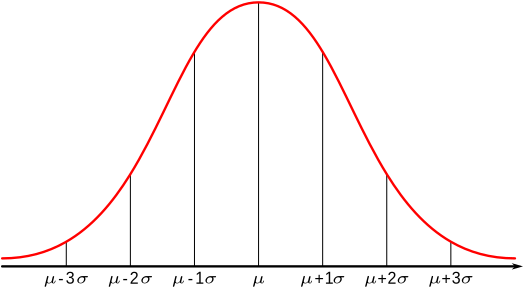
\includegraphics[width=0.65\linewidth]{\currentDir/normalDistPdf}%
\caption{A sketch of the probability density function of the normal distribution given in \cref{eq:normalDistributionPdf}.}%
\label{fig:normalDistPdf}%
\end{figure}%
%
Here, $\mu$~is the arithmetic mean, i.e., the expected value, of the distribution and $\sigma$~is its standard deviation~(making $\sigma^2$~its variance).
$x$~is the variable of this function.
This function describes typical bell-shaped curve of the normal distribution as sketched in \cref{fig:normalDistPdf}.
Implementing this function as a, well, function in \python\ is straightforward.
\Cref{lst:functions:normal_pdf}\pythonIdx{pi}\pythonIdx{exp}\pythonIdx{sqrt} offers the function \pythonil{pdf} with three parameters: \pythonil{x}, \pythonil{mu}, and~\pythonil{sigma}, which represent~$x$, $\mu$, and~$\sigma$.%
%
\begin{sloppypar}\pythonIdx{function!call}%%
Now, the two parameters~$\mu$ and~$\sigma$ of~$f$ (respectively~\pythonil{mu} and~\pythonil{sigma} of~\pythonil{pdf}) represent the general normal distribution.
The \emph{standard} normal distribution has $\mu=0$ and $\sigma=1$, i.e., is centered around the mean~$0$ and has a standard deviation (and variance) of~$1$.
We therefore define the \emph{default} values for \pythonil{mu} to be~\pythonil{0.0} and for \pythonil{sigma} to be~\pythonil{1.0}.
This is done directly in the header of the function.
Instead of writing \pythonil{x: float, mu: float, sigma: float}, we write \pythonil{x: float, mu: float = 0.0, sigma: float = 1.0}.%
\end{sloppypar}%
%
In \cref{lst:functions:use_normal_pdf}, we import our new \pythonil{pdf} function and use it inside a program.
When calling \pythonil{pdf}, we can omit the values of the parameters with default values, in which case they will take on their default values.
For example, invoking \pythonil{pdf(0.0)} if equivalent to calling~\pythonil{pdf(0.0, 0.0, 1.0)}.
We also can specify some of the parameters with default values while omitting others.
For instance, the function call \pythonil{pdf(2.0, 3.0)} is the same as \pythonil{pdf(2.0, 3.0, 1.0)}.
Obviously, we must always specify the first parameter~(\pythonil{x}), because it has no default value.%
%
\bestPractice{defaultValues}{%
\pythonIdx{function!parameter!default value}\pythonIdx{function!argument!default}%
Default parameter values must always be immutable.}%
%
The default value of a function must always be immutable.
If you would pass in, e.g., a \pythonil{list}, then the function could modify the list and the next call to this function would then receive this modified list.
Even worse, if the function was to return the list, it could be modified outside of the function.
The behavior of such code could become arbitrarily hard to debug.

Back to business.\pythonIdx{function!parameter!by name}\pythonIdx{function!argument!by name}
What would we do if we want to specify the value of the parameter \pythonil{sigma} of our function, but leave \pythonil{mu} at its default value?
We can do this by passing in values by parameter name:
\pythonil{pdf(-2.0, sigma=3.0)}~passes in \pythonil{-2.0} for~\pythonil{x} and \pythonil{3.0} for~\pythonil{sigma}.
It does not specify any value for~\pythonil{mu}, leaving it at its default value, which renders the call equivalent to~\pythonil{pdf(-2.0, 0.0, 3.0)}.
This passing in of arguments by specifying \pythonil{parameterName=value} also allows us to specify the arguments in arbitrary order.
\pythonil{pdf(mu=8.0, x=0.0, sigma=1.5)} is an example of this.
Don't do such things, though.%
%
\begin{sloppypar}%
\Cref{lst:functions:use_normal_pdf} provides also another interesting way to call a function in \python.
As we have established by now, the parameters of a function have names.
If we write something like \pythonil{mu=8.0, x=0.0, sigma=1.5} to assign arguments, this looks very similar to the way we created dictionary constants back in \cref{sec:dictionaries} and \cref{lst:dicts:dicts_1}.
Calling \pythonil{pdf(-2.0, sigma=3.0)} is equivalent to writing~\pythonil{pdf(x=-2.0, sigma=3.0)}.%
\end{sloppypar}%
%
We can create a dictionary with the values \pythonil{\{"x": -2.0, "sigma": 3.0\}}.
Let's call this dictionary~\pythonil{args_dict}.
Can we now somehow pass in these values to~\pythonil{pdf}?
We indeed can:
We just have to write~\pythonil{pdf(**args_dict)}.\pythonIdx{**!function parameter}\pythonIdx{function!parameter!**}\pythonIdx{function!argument!**}\pythonIdx{function!argument!keyword}\pythonIdx{dict}
Doing this will unpack the dictionary \pythonil{args_dict} and pass all the values under their assigned names in as arguments to their corresponding parameters.
\pythonil{pdf(**args_dict)} is thus equivalent to~\pythonil{pdf(x=-2.0, sigma=3.0)}.
Two things are to notice here:
First, the double~\pythonil{*}\pythonIdx{*!function parameter}\pythonIdx{function!argument!*}\pythonIdx{function!parameter!*} (called %
wildcard\pythonIdx{wildcard}\pythonIdx{function!argument!wildcard}\pythonIdx{function!parameter!wildcard}, %
star\pythonIdx{star}\pythonIdx{function!argument!star}\pythonIdx{function!parameter!star}, or %
asterisk\pythonIdx{asterisk}\pythonIdx{function!argument!asterisk}\pythonIdx{function!parameter!asterisk}) %
\emph{before} the dictionary, i.e., the~\pythonil{**}\pythonIdx{**!function parameter} is telling \python\ to unpack the dictionary this way.
Second, default argument values still apply here, i.e., \pythonil{mu} will have value~\pythonil{0.0} in this function call.

Similarly, maybe we do not care about the parameter names but want pass them in by position, as we have always done in the past.
Then, we can construct a sequence, e.g., a \pythonilIdx{list} or \pythonilIdx{tuple} with the parameter values.
Of course, \pythonilsIdx{list} and \pythonilsIdx{tuple} do not store key-value relationships, only values at positions.
We could create a tuple~\pythonil{args_tuple} with the value~\pythonil{(-2.0, 7.0, 3.0)}.
Then, invoking \pythonil{pdf(*args_tuple)} will basically fill in the three values in their into the parameters, i.e., will be equivalent to~\pythonil{pdf(-2.0, 7.0, 3.0)}.
This time, only a single wildcard~\pythonil{*}\pythonIdx{*!function parameter}\pythonIdx{function!argument!*}\pythonIdx{function!parameter!*} is placed before~\pythonil{args_tuple}.
We can also pass the parameters in by \inQuotes{unpacking} a list.
In our example \cref{lst:functions:use_normal_pdf}, we create the list \pythonil{args_list = [2.0, 3.0]}.
Calling~\pythonil{pdf(*args_list)} then is the same as writing~\pythonil{pdf(2.0, 3.0)}, which, in turn, is identical to~\pythonil{pdf(2.0, 3.0, 1.0)}.
Again, parameters with default values do not need to be supplied.

At first glance, the use of all of the above is not entirely clear.
What do we need default parameter values for?
Well, in some cases, you may want to enable a user to \inQuotes{customize} your functions.
A typical example is the \href{https://matplotlib.org/stable/api/_as_gen/matplotlib.axes.Axes.plot.html}{\pythonilIdx{plot} method} of the \pythonilIdx{Axes} object provided by popular \matplotlib\ library.
You will normally provide a sequence of x-\ and y\nobreakdashes-coordinates to this function it will draw a line which goes through all the points specified this way.
However, you can also optionally specify a color for the line, markers to be painted at the points, line dash style, a label, colors and sizes for the markers, a z\nobreakdashes-order to be used if multiple lines are drawn, and so on, and so on.
The use of default arguments allows the function call to be relatively simple in most cases, while still allowing the user to do more complex formatting if need be.

From this example, we can also directly extrapolate a use case for building the arguments of a function in a dictionary.
Imagine that you write an own function that uses one of the plotting methods of \matplotlib.
Let's say that your function does a plot call where it provides ten parameter values.
However, you have one special case where you need to provide one more parameter, maybe a line dash style that you otherwise do not need to provide.
Then, you could have some \pythonil{if} in your code that branches to do the ten-parameter-call in one case and the eleven-parameter-call in the other.
This means that a rather complex function call appears twice in a very similar manner.
If you instead construct the parameters in a dictionary and in the \pythonil{if} branch just add the eleventh parameter if need be, your code will become much simpler.%
%
\FloatBarrier%
\endhsection%
%
\hsection{Functions as Parameters or Variables, \texttt{Callable}, and \texttt{lambda}s}%
\label{sec:functionsAsVarsAndLambdas}%
%
We have just learned that we can basically construct a function call by placing the parameter values into collection objects and then invoke the function by \inQuotes{unpacking} the collection using either \pythonil{*} (for position-based parameters) or \pythonil{**} (for dictionaries).
But there is one more interesting thing that we can do with functions.
You see, in \python, all things are objects.
References to objects can be stored by variables or passed in as function arguments.
Functions are objects too.
This means that we can also store functions in variables or pass them as argument to other functions!

At first glance, this sounds awfully odd.
Why would someone like to pass a function as parameter to another function?
At second glance, there are a wide variety of situations where we would actually want to do that.
Having done so many mathematics-based examples in this book, let's pick one such situation arising in maths.

In high school, you have learned about integration and differentiation.
A \emph{definite integral} is the formal calculation of the area under a function, using infinitesimal stripes of the region.
The second fundamental theorem of calculus states:
Given a function~$f(x)$ which is continuous over the real interval~$[a,b]$ and its antiderivative~$F(x)$, the definite integral $\int_a^b f(x)\,dx = F(b)-F(a)$ (where antiderivative means that~$F'=f$).
In other words, if we want to get the area beneath~$f(x)$ over the interval~$[a,b]$, we would first obtain the antiderivative and then simply calculate~$F(b)-F(a)$.
Obtaining the antiderivative involves pen and paper symbolic maths.
We cannot really program such maths at this stage in this book as an example.
But we can go back to the original definition of the definite integral, namely that it equals the area beneath the function obtained by using infinitesimal (read:~immeasurably small) strips of the region.

While we cannot really use \inQuotes{immeasurably small} strips, we could use \inQuotes{fairly small} ones to approximate the right result.
If we have a function~$f(x)$, which would obviously be a parameter of our program, as well as the interval limits~$a$ and~$b$, we could divide the range~$[a,b]$ into~$n$ strips.
For each strip, we could approximate the area beneath~$f(x)$, add up the~$n$ areas, and have a rough approximation of the total area.
$n$~could be another parameter for our integration approach:
The larger~$n$, the smaller will the strips get, the more accurate should our estimate become (and the longer it will take to get it).%
%
\begin{figure}%
\centering%
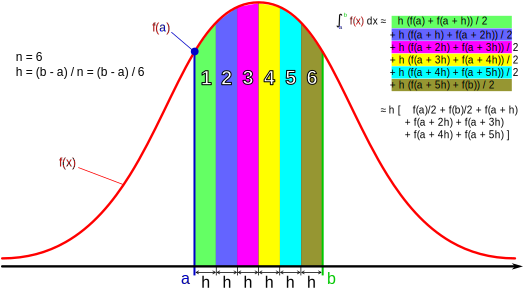
\includegraphics[width=0.65\linewidth]{\currentDir/normalDistPdfInteg}%
\caption{A sketch of the trapezoid method for approximating definite integrals.}%
\label{fig:normalDistPdfInteg}%
\end{figure}%
%
\gitPythonAndOutput{\programmingWithPythonCodeRepo}{05_functions}{integral.py}{--args format}{functions:integral}{%
Using the trapezoid method to numerically approximate definite integrals, as sketched in \cref{fig:normalDistPdfInteg}.}%

The trapezoid method is one very simple implementation of this idea~\cite{E2013AITNMAA}.
As illustrated in \cref{fig:normalDistPdfInteg}, it treats the strips as right trapezoids.
The baseline of the trapezoid is a piece of the \pgls{xAxis} with length~$h=(b-a)/n$.
Clearly, $n*h=b-a$ and thus, $n$~trapezoids of equal base length form the range of the \pgls{xAxis} under~$f(x)$.
The baseline first trapezoid starts right at~$x=a$ and extends to~$x=a+h$.
The second trapezoid starts at~$x=a+h$ and extends to~$x=a+2h$.
The last trapezoid starts at~$x=a+(n-1)h$ and extends to~$x=a+nh=b$.
Each trapezoid has two sides meeting with its baseline in right angles.
The length of these sides are the values of~$f(x)$ at the corresponding x\nobreakdashes-coordinate.
The area of the $i$\nobreakdashes-th trapezoid is thus~$h[f(a+(i-1)h)+f(a+ih)]/2$.
Summing up the $n$~areas yields an approximation of the definite integral, as sketched in \cref{fig:normalDistPdfInteg}.

Each value~$f(a+ih)$ except for $i=0$ and $i=n$ appears twice in the sum and each time is halved.
Instead of computing these values twice, dividing them by two, and then adding them, we can simply compute them only once.
Our implementation \pythonil{integrate} of this approach, given in \cref{lst:functions:integral}, does exactly that.

The interesting part of our \pythonil{integrate} method, however, is not the approximation of the integral.
It is the header.
More precisely, it is the first parameter:~\pythonil{f: Callable[[float], float | int]}\pythonIdx{Callable}\pythonIdx{typing}.
\pythonilIdx{Callable} is the \pgls{typeHint} for anything that can be called, i.e., functions~\cite{PSF2024ACO}.
Like the \pgls{typeHint} for lists and tuples, it can be parameterized following the scheme~\cite{PEP612}:%
%
\begin{pythonSyntax}
Callable[[parameterType1, parameterType2, ...], resultType]
\end{pythonSyntax}
%
In other words, inside the \pythonil{Callable[...]}, we first provide the list of parameter types, then a comma~\pythonil{,} followed by the return type.
\pythonil{f: Callable[[float], float | int]} thus states that our function expects, as first parameter, \emph{another function}~\pythonil{f}.
\pythonil{f}~must accept one parameter of type~\pythonil{float}.
Its return type is \pythonil{float | int}, i.e., it should return either a~\pythonil{float} or~\pythonil{int}\pythonIdx{\textbar!type hints}~\cite{PEP604}.
Notice that the type \pythonilIdx{Callable} is provided by the module~\pythonilIdx{typing}\footnote{%
\cite{PSF2024ACO}~states that this import is now deprecated and we should use \pythonil{collections.abc.Callable}\pythonIdx{collections.abc} instead. %
In the past, this created some errors for me, so for now we stick with using~\pythonilIdx{typing}.}, %
so we need to import it first if we want to use it.%
%
\begin{sloppypar}%
Additionally, our \pythonil{integrate} function accepts two parameters~\pythonil{a} and~\pythonil{b} which must be of type~\pythonil{float | int}, i.e., can either be an \pythonil{float} or \pythonil{int}.
Their default values are~\pythonil{0.0} and~\pythonil{1.0}, meaning that we will integrate over~$[0,1]$ if they are not specified.
As final parameter, we expect an integer~\pythonil{n}, by default~\pythonil{100}, which corresponds to the number of trapezoids that we shall use for the approximation.%
\end{sloppypar}%
%
Let's now test how well our trapezoid-based integration works.
First, let's compute the definite integral~$\int_0^1 1\,dx$.
For this purpose, we need to pass the function~$f(x)=1$ as the~\pythonil{f} parameter of~\pythonil{integrate}.
We could do this by writing:%
%
\begin{pythonSyntax}
def const_1(x: float) -> float:
    return 1.0
\end{pythonSyntax}
%
or%
%
\begin{pythonSyntax}
def const_1(_: float) -> float:
    return 1.0
\end{pythonSyntax}
%
where the \pythonil{_}\pythonIdx{\_} indicates that we are actually going to ignore this parameter~(see~\cref{bp:underscore}).
We could then invoke~\pythonil{integrate(const_1)}.

However, there also is a more compact way to specify functions that we are only going to use once:
The so-called \pythonilsIdx{lambda}~\cite{PSF2024L}, which have the structure%
%
\begin{pythonSyntax}
lambda param1, param2, ...: return value
\end{pythonSyntax}
%
Due to the \pythonilIdx{:} in the notation, we cannot annotate \pythonilsIdx{lambda} with \pglspl{typeHint}.
As a \pythonil{lambda} expression is very small and only used once, this does not pose a serious problem.
Either way, since we need one parameter for our 1-returning-function and since we do not care about the value of this parameter, we can simply write:%
%
\begin{pythonSyntax}
integrate(lambda _: 1.0)
\end{pythonSyntax}
%
\pythonilsIdx{lambda} are functions that we only want use in a single place.
This is clearly the case for a function that ignores its parameter and always returns~\pythonil{1.0}.
So we pass this expression into our \pythonil{integrate} function as value of the parameter~\pythonil{f}.

Obviously, the area under the constant function~$1$ over the range~$[0,1]$ is also~$1$.
Using \pythonil{n=7} trapezoids, we get exactly this result.
In the output of our program, we write~\inlinelistingbox{$\int$\lstinline[style=text_style]$1dx|0,1$} where the~\textil{|0,1} denotes the limits~$[0,1]$ of the interval over which we integrate (and we use the unicode escape \pythonil{"\\u222b"} to represent the~$\int$~character in the \pglspl{fstring}).

Having passed this simple sanity test, let's try to compute the beneath under the function~$g(x)=x^2-2$ over the interval~$[-1,1]$, i.e.,~$\int_{-1}^1 x^2-2\,dx$.
The antiderivative of~$g(x)$ is~$G(x)=\frac{1}{3}x^3-2x+c$ and $G(1)-G(-1)=[\frac{1}{3}-2]-[-\frac{1}{3}+2]=\frac{2}{3}-4=-3\frac{1}{3}=-3.\overline{3}$.
We pass the function~$g(x)$ as \pythonil{lambda} expression into our \pythonil{integrate} function by writing~\pythonil{lambda x: x*x - 2}.
We also need to specify a value for the parameter~\pythonil{a}, namely~\pythonil{-1}.
Using the default value of \pythonil{n=100} steps, our method returns~\pythonil{-3.3332}, which is fairly close to~$-3.\overline{3}$.

Let us now integrate the sinus function over the interval~$[0,\numberPi]$.
We can import~\pythonilIdx{sin} from the \pythonilIdx{math}~module and pass it into our function for~\pythonil{f}.
We also need to specify \pythonil{b = pi}\pythonIdx{pi}, which we, too, have imported from~\pythonilIdx{math}.
This time, we use \pythonil{n = 200} trapezoids to approximate the definite integral.
The antiderivative of~$\sin x$ is~$-\cos x+c$, so the expected output would be~$[-\cos\pi]-[-\cos 0]=[-(-1)]-[-1]=2$.
Indeed, our function delivers about~$1.99996$, which is, again, fairly close.

Let us, as final example, also integrate the probability density function~(PDF) of the normal distribution.
We implemented this function and called it \pythonil{pdf} back in \cref{lst:functions:normal_pdf}, so we just need to \pythonilIdx{import} it from there.
Notice that this function actually had three parameters, \pythonil{x}, \pythonil{mu}, and~\pythonil{sigma}.
The latter two had the default values~\pythonil{mu = 0.0} and~\pythonil{sigma = 1.0}.
If these values are used, the function computes the PDF of the \emph{standard} normal distribution.

\gitOutputTool{\programmingWithPythonCodeRepo}{.}{scripts/mypy.sh 05_functions integral.py}{functions:integral:mypy}{%
The results of static type checking with \mypy\ of the program given in \cref{lst:functions:integral}.}

Interestingly, although we demand that the function supplied to \pythonil{integrate} should only have one parameter, we can still pass in~\pythonil{pdf} due to its second and third parameter being optional.
Even \mypy\ accepts this function as valid parameter, as its output (or better, the lack of it) in \cref{exec:functions:integral:mypy} suggests.

The standard normal distribution has standard deviation~$\sigma=1$ and mean~$\mu=0$.
If we integrate it over the interval~$[-1,1]$, we basically compute the probability that a standard normally distributed random variable~$X$ is drawn from the interval~$[\mu-\sigma,\mu+\sigma]$, i.e., from within one standard deviation from the mean.
As you may still know from high school math, this probability is roughly~68.26\%.
Similarly, the probability that such a random variable is sampled from within~$[-2,2]$, i.e., not more than two standard deviations away from the mean, is about~95.44\%.
The output of our little integrator function in \cref{exec:functions:integral} fits perfectly to this.

As a final clarification, let us mention that trapezoid-based approximation of definite integrals is by no means the best approach.
Others, like Simpson's rule, are much better~\cite{E2013AITNMAA}.
Still, as an example of functions that work on other functions, it was suitable.%
\FloatBarrier%
\endhsection%
%
\hsection{Summary}%
Functions are the central building block needed to create modular code.
They allow us to put code into units with clearly defined interfaces.
The input of a function are its parameters~(if any).
The output is its return value~(if any).
Both parameters and return value can be annotated with \pglspl{typeHint}.
The description of what the function does as well as what the parameters and the return value mean, goes into the \pgls{docstring}.

This clear definition and separation from the rest of the code has several advantages.
First, multiple programmers can work together on a project.
They can work on different functions, which we can place into different modules~(\python\ files).
If we did not have functions available, this would be impossible.

Second, by using proper \pglspl{typeHint} for the function parameters and return value as well as proper \pglspl{docstring}, the behavior of functions is easier to understand by fellow programmers.
Type checkers like \mypy\ can also verify whether functions are called with correct parameters more easily.
The code does not just become more modular, but easier to maintain.
It can be checked by static code analysis tools as well.

Third, functions allow us to reuse pieces of code in different locations.
If we want to compute the definite integral of two different functions, we do not have to implement two routines for integration.
We can make one and use it in two different locations.

Fourth, if we have a code with clearly defined input and output that exists in isolation from other code, then we can \emph{test} this code in isolation as well.
It may be extremely difficult to test a complete program.
However, it may be rather straightforward to test a small function.
Unit tests, for example using the \pytest\ framework, allow us to do just that.
It is also not hard to imagine that unit tests can compound our trust into our code:
In the previous sections, we developed a function~\pythonil{pdf} for computing the probability density function of the normal distribution and a function~\pythonil{integrate} for approximating definite integrals.
Assume that we properly unit tested these two functions and shown for both of them that they produce the expected results for a wide range of different inputs.
It would be easy to see that this then would also give us a certain confidence that using \pythonil{integrate} to compute a definite integral over a certain input range of~\pythonil{pdf} should be correct, too.
This could be verified with some additional unit tests.
Working our way up from testing small components to larger and larger building blocks of an application gives us a good chance to have only few bugs in the final product.

These are a lot of advantages of using functions.
But functions in \python\ also come with lots of nice features as well.

For example, we can specify default values for function parameters.
This allows us to create functions that can be invoked using only few arguments in the normal case and that can be customized with more parameters in special cases.
Since functions themselves are objects, they can be stored in variables and parameters as well.
The proper \pgls{typeHint} for such variables or parameters is defined using the~\pythonilIdx{Callable} type.
Functions that accept \pythonilsIdx{Callable} as parameter can also accept \pythonilsIdx{lambda}.
\pythonilsIdx{lambda} are an abbreviated way to define functions, usually in a single line and only for a single use.%
\endhsection%
%
\endhsection%
%
